\documentclass[hidelinks,12pt]{article}
\usepackage{amsmath}
\usepackage{graphicx}
\usepackage[english]{babel}
\usepackage[utf8]{inputenc}
\usepackage{fancyhdr}
\usepackage{tabularx}
\usepackage{hyperref}
\usepackage{float}
\usepackage{subcaption}
\usepackage{listings}
\usepackage{xcolor}

\definecolor{codegreen}{rgb}{0,0.6,0}
\definecolor{codegray}{rgb}{0.5,0.5,0.5}
\definecolor{codepurple}{rgb}{0.58,0,0.82}
\definecolor{backcolour}{rgb}{0.95,0.95,0.92}

\lstdefinestyle{mystyle}{
    backgroundcolor=\color{backcolour},   
    commentstyle=\color{codegreen},
    keywordstyle=\color{magenta},
    numberstyle=\tiny\color{codegray},
    stringstyle=\color{codepurple},
    basicstyle=\ttfamily\footnotesize,
    breakatwhitespace=false,         
    breaklines=true,                 
    captionpos=b,                    
    keepspaces=true,                 
    numbers=left,                    
    numbersep=5pt,                  
    showspaces=false,                
    showstringspaces=false,
    showtabs=false,                  
    tabsize=2
}

\lstset{style=mystyle}

\hypersetup{
    colorlinks=true,
    linkcolor=cyan,
}

\pagestyle{fancy}
\fancyhf{}
\chead{Postfix Evaluator in MIPS}
\rfoot{\thepage}

\begin{document}

\begin{titlepage}
    \centering
    
\includegraphics[scale=0.5]{../../logo.png}\\[1.0cm]
    \Large INDIAN INSTITUTE OF TECHNOLOGY DELHI\\[1.0 cm]
    \LARGE COL216\\[0.1cm]
    \Large \underline{Report}\\
    \large \[Assignment-1\]
    \LARGE \textbf{Postfix Evaluator in MIPS}
    

    \rule{\textwidth}{0.2 mm} \\[0.1cm]
    \begin{abstract}
        This program evaluates a postfix expression of digits using a stack based algorithm.
        This has been written in MIPS assembly language to better understand the hardware abstractions.
                \\[0.1cm]    
    \end{abstract}
    \rule{\textwidth}{0.2 mm} \\[0.1cm]
    \begin{flushright}
        
        \begin{tabular}{c c}
            \small {Harsh Agrawal} & \small {2019CS10431} \\
            \small {Saptarshi Dasgupta} & \small {2019CS50447} \\
        \end{tabular}
    \end{flushright}
\end{titlepage}
\tableofcontents
\newpage

\section{Approach}
We implemented a stack based algorithm to evaluate the input postfix expression. The algorithm is as follows

\subsection{Algorithm}
The algorithm iterates over the input string character by character
\begin{enumerate}
    \item When the current character is an operand $(0-9)$ the character is pushed to the program stack.
    \item When the current character is an operator $(+|-|*)$ the top two entries in the stack are popped and the corresponding operation is performed. The result of the operation is pushed back to the stack.
    \item When the current character is either a newline $(\symbol{92}n)$ or the null character $(\symbol{92}x00)$ the topmost entry is popped from the stack and printed.
\end{enumerate}

\subsection{Efficiency}
The above algorithm iterates over the input string only once and in a single pass is able to evaluate the expression.
Hence the asymptotic time complexity of the algorithm is $O(n)$ where $n$ is the length of the input string.


\section{Testing}
We employed both automated and manual modes of testing. The automated mode helped establish the correctness whereas the manual mode helped handle the corner cases.
\subsection{Automated}
We wrote a \verb|python3| script that generates random postfix expressions, executes the asm file in a MIPS emulator (\verb|spim|), communicates with the executed process through unix pipes, and compares the
output with the expected value. To install the dependencies, enter the following commands once inside root project folder.
\begin{lstlisting}[language=bash]
    $ sudo apt install spim
    $ python3 -m pip install -r requirements.txt
    $ python3 tester.py -n 20 -k 30 
\end{lstlisting}
The last command will run $20$ test cases with $30$ operands in each test case and print a test log with all the test cases generated and the result of each test case.

\subsection{Manual}
We have provided the functionality to run custom test cases so that corner cases may be tested for. We can either write the test cases into a file or provide the values on \verb|STDIN|.
\begin{lstlisting}[language=bash]
    $ python3 tester.py -i <testcase_file_path>
\end{lstlisting}
This will read the test cases from input file. If test cases are to be provided on \verb|STDIN|, use the below command.
\begin{lstlisting}[language=bash]
    $ python3 tester.py --manual
\end{lstlisting}
\subsection{Results}
The test case logs are provided in the \verb|./tests| directory. This includes both the automatically generated test cases as well as the manual test cases. Based on the logs we conclude the following:
\subsubsection{Automated}
The execution logs for these test cases are stored in the \verb|./tests/automated| directory.
\begin{enumerate}
    \item When the number of operands were less, most of the test cases passed.
    \item All the test cases that failed were those which included integer overflows. The result of the postfix expression exeeded the integer bounds of a 32 bit register.
\end{enumerate}
\subsubsection{Manual}
The execution logs for these test cases are stored in the \verb|./tests/manual| directory.
\begin{enumerate}
    \item \verb|extra_operands|: The postfix expression had more operands making it an invalid postfix expression. In this test case our code raised a exception.
    \item \verb|extra_operators|: The postfix expression had more operators than operands to operate upon. In this case our program raised an exception.
    \item \verb|invalid_operand|: The operand was not a digit and our program raised an exception since it cannnot operate on a non-numeric input.
    \item \verb|invalid_operator|: The operators are restricted to $(+|-|*)$. Any other character is flagged as an illegal character and an exception is raised.
    \item \verb|invalid_postfix|: The postfix expression is invalid, in such case our program generated an appropriate exception.
    \item \verb|empty_input|: The input string was empty, in this case our program generated the output $0$.
    \item \verb|overflow|: These test cases explicitly introduce arithmetic overflow in computations. Our program generates an arithmetic overflow exception for such cases.
\end{enumerate}
\begin{figure}[h!]
    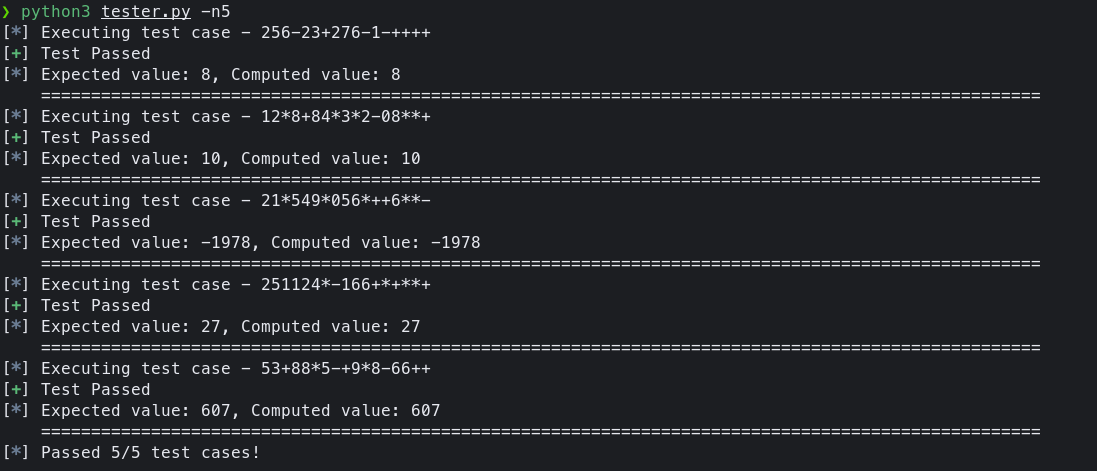
\includegraphics[width=\linewidth]{logs.png}
    \caption{Automated Testing example}
    \label{fig:boat1}
\end{figure}

\subsubsection{Efficiency}
We tested the efficiency of our program execution. We plotted the above graph with execution time on the y axis and the length of the input string on the axis.
We found that the graph came out to be a straight line, indicating that the time complexity of the procedure is $O(n)$


\begin{figure}[h!]
    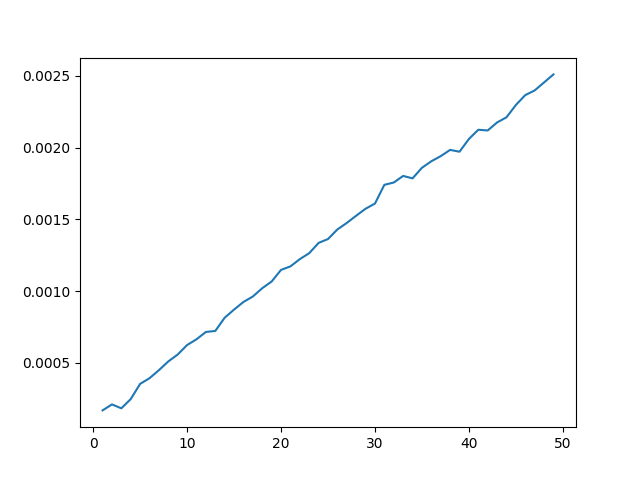
\includegraphics[width=\linewidth]{timing.png}
    \caption{Graph of Execution time vs. Number of Operands}
    \label{fig:boat1}
\end{figure}

\section{Assumptions}
\begin{itemize}
    \item The size of input string is capped at \verb|8 KB|, which is equivalent to $8192$ characters. This design decision was made to ensure that the input string does not cause a stack overflow.
    \item We have assumed that the digits are one of $(0-9)$ and the operands are $(+|-|*)$, any other operator or operand is flagged as illegal character and appropriate exceptions are raised.
    \item We make the assumption that the result of the postfix expression will not lead to an integer overflow. This means our program is capable of evaluating only those expressions that are within the bounds $[-2^{31}, 2^{31}-1]$
    \item Lastly we assume that the logic for evaluating the postfix expression in tester script is correct since it is fairly easy to code it in a high level programming language like python than a low level programming language like assembly.
\end{itemize}

\end{document}

